\documentclass[a4paper,10pt,oneside]{memoir}

%\usepackage{Packages}

\ProvidesPackage{Packages}

\usepackage{a4wide}
\usepackage{amsmath}
\usepackage{fancyhdr}
\usepackage{gensymb}
\usepackage{graphicx,wrapfig}
\usepackage{grffile}
\usepackage{pifont}
\usepackage{float}
\usepackage[italian]{babel}

\usepackage{caption}
\captionsetup{format=plain, labelfont=bf, skip=0pt}

\usepackage{paralist}
\usepackage[usenames,dvipsnames]{color}
\usepackage{moreverb}
\usepackage{lscape}
%\usepackage[nottoc]{tocbibind}
\usepackage{verbatim}
\usepackage{datetime}
\usepackage{array}

\usepackage{color}
\definecolor{darkred}{rgb}{0.5,0,0}
\definecolor{darkgreen}{rgb}{0,0.5,0}
\definecolor{darkblue}{rgb}{0,0,0.5}
\definecolor{gray}{rgb}{0.35,0.35,0.35}

\usepackage[pagebackref=true,
            colorlinks=black,
            linkcolor=gray,
            bookmarks=true,
            filecolor=gray,
            urlcolor=gray,
            citecolor=gray
           ]{hyperref}

%\usepackage{titlesec}


%\titlespacing\section{0pt}{12pt plus 4pt minus 2pt}{0pt plus 2pt minus 2pt}
%\titlespacing\subsection{0pt}{12pt plus 4pt minus 2pt}{0pt plus 2pt minus 2pt}
%\titlespacing\subsubsection{0pt}{12pt plus 4pt minus 2pt}{0pt plus 2pt minus 2pt}

\usepackage{chngcntr}
\counterwithout{section}{chapter}

\usepackage{tocloft}


\usepackage{inputenc}
\usepackage{tikz}
\usepackage{anysize}
\usepackage{color} 
\marginsize{1.5cm}{1cm}{1cm}{2cm}
\usepackage[siunitx,european,americanresistors]{circuitikz}
\definecolor{logo}{HTML}{158388}
\definecolor{logo2}{HTML}{FFFFFF}
\definecolor{scritta}{HTML}{000000}

\def\sectionfont{\bfseries\LARGE}
\def\subsectionfont{\bfseries\Large}

%\renewcommand\cftsectionaftersnumb{\textbf}
\renewcommand{\cftsectionfont}{\normalfont\bfseries}% titles in bold

\usepackage{lipsum}


\setlength\cftsectionindent{0pt}
\setlength\cftsubsectionindent{15pt}
\setlength\cftsectionnumwidth{2em}
\setlength\cftsubsectionnumwidth{4em}

\renewcommand\cftbeforesectionskip{7pt plus 1pt}
\renewcommand\cftbeforesubsectionskip{4pt plus 1pt}

%\renewcommand\cftsecfont{\Large\bfseries}
%\renewcommand\cftsubsecfont{\large\bfseries}

%\renewcommand\cftsecpagefont{\large\bfseries}
%\renewcommand\cftsubsecpagefont{\large\bfseries}

%\renewcommand\cftsecafterpnum{\par\addvspace{15pt}}
%  \renewcommand\cftsubsecafterpnum{\par\addvspace{15pt}}



\usepackage{lineno}
\usepackage{longtable}
\usepackage[section]{placeins}
\usepackage{url}
\usepackage{makeidx}
\usepackage{hyperref}
\usepackage{subfig}

\usepackage{booktabs}
\usepackage{rotating}
\usepackage[absolute]{textpos}

\usepackage{listings}


\setlength{\parindent}{0.0in}
\setlength{\parskip}{0.1in}
\setlength{\marginparwidth}{2.3cm}

\newcommand\todo[1]{
  \-\marginpar[\raggedleft\footnotesize #1]
  {
    \raggedright\footnotesize #1
  }
}

\newcommand\ltodo[1]{
  \-\marginpar[\raggedleft\footnotesize ]
  {
    \raggedright\footnotesize
  }
}

%\docdate
%\newcommand{\docdate}{\today}

%\newcommand{\clearemptydoublepage}{
%    \newpage{\pagestyle{empty}
%    \cleardoublepage}
%}

\fancypagestyle{plain}{
\fancyhf{}
\fancyfoot[LO,RE]{\doctitle}
\fancyfoot[RO, LE]{\thepage}
\renewcommand{\headrulewidth}{0pt}
\renewcommand{\footrulewidth}{0.4pt}}

\pagestyle{plain}

\modulolinenumbers[5]

\newcommand{\tick}{\textcolor{darkgreen}{\ding{51}}}
\newcommand{\cross}{\textcolor{darkred}{\ding{55}}}
\usepackage[framed,numbered,autolinebreaks,useliterate]{Listings}


\addto\captionsbritish{\renewcommand{\contentsname}{Indice}}

%\linenumbers

\newcommand{\researchgroup}{LABORATORIO DI FISICA I}

\newcommand{\doctitle}{Laboratorio di Fisica - Esperienza di Elettromagnetismo}

\begin{document}
\counterwithout{figure}{chapter}
\counterwithout{figure}{section}
% SECTIONS
\makeatletter
\setsecheadstyle{\tikz{
\fill[logo](1,-1.85) rectangle (14,-2);
\node[inner sep=0pt,outer sep=0pt,text=white,scale=1.5,font=\sectionfont]  at (.5,-1.35) {\color{scritta}\Large\thesection};

    
}\vskip-9ex\hskip5em\sectionfont\color{scritta}}
% SUBSECTIONS
\setsubsecheadstyle{\tikz{
\fill[logo](1.5,-3.90) rectangle (8,-4);
\node[inner sep=0pt,outer sep=0pt,text=logo,scale=1,font=\sectionfont]  at (.5,-3.43)  {\color{scritta}\quad\thesubsection};
\node[inner sep=0pt,outer sep=0pt,text=logo2,scale=1,font=\sectionfont]  at (1.6,-3.5){$\gg$};
}\vskip-8ex\hskip5em\subsectionfont\color{scritta}
}
\setcounter{tocdepth}{2}
\setcounter{secnumdepth}{2}% to number subsubsections

\def\@seccntformat#1{\hskip0em}
\makeatother

\setbeforesecskip{\onelineskip}
\setaftersecskip{2\onelineskip}



\setbeforesubsecskip{-1\onelineskip}
\setaftersubsecskip{2\onelineskip}


\setbeforesubsubsecskip{-1\onelineskip}
\setaftersubsubsecskip{3\onelineskip}



\pagenumbering{gobble}
\begin{center}
\vspace*{5.8cm}

\setlength{\TPHorizModule}{1mm}
\setlength{\TPVertModule}{\TPHorizModule}

\newlength{\backupparindent}
\setlength{\backupparindent}{\parindent}
\setlength{\parindent}{0mm}

\begin{textblock}{155}(30,20)
    \vspace*{1mm}
    \huge
    \textbf{Esperienza di Elettromagnetismo\\}
    \LARGE
    \vspace*{5mm}
    Verifica sperimentale della forza di Lorentz.
    \textbf{}
    \par
    \vspace*{15mm}
    \Large
    \begin{textblock}{155}(30,60)
    \begin{flushleft}
        \Large
           
            
             \textbf{Componenti:} Vittorio Strano, Arianna Genuardi, Florinda Tesi, Antonio Riolo, Matteo Romano
            
            
            

    \end{flushleft}
    \end{textblock}
\end{textblock}

\setlength{\parindent}{\backupparindent}
\end{center}

\tableofcontents*

\newpage
\normalsize
\pagenumbering{arabic}
\section{Introduzione}
{\fontsize{12}{14}\selectfont 

Lo scopo dell'esperimento è quello di verificare la relazione tra la forza di Lorentz applicata ad un circuito immerso in un campo magnetico B al variare della corrente I, della lunghezza del circuito L e dell'angolo $\theta$ che esso forma con il campo magnetico.

\par

La relazione che lega il modulo della forza di Lorentz a queste grandezze è:

\begin{equation}\label{eq:FL}
  F_L = LIB\sin(\theta)
\end{equation}

\par}
 

\section{Metodi sperimentali}
\subsection{Strumentazione}
{\fontsize{11}{14}\selectfont 
Gli strumenti utilizzati in questa esperienza sono:
\begin{enumerate}
    \item \textbf{Generatore DC Cosmo 3000}
    \item \textbf{Current Balance Main Unit}
    \item \textbf{Accessory Unit} con un errore di mezza tacca sul goniometro, $\delta_{\theta} = 0.5$°
    \item \textbf{Magnete A} largo abbastanza da poter inserire al suo interno i circuiti stampati 
    \item \textbf{Magnete B} utilizzato insieme all'accessory unit.
    \item \textbf{Sei differenti circuiti stampati} con valori tabulati. Alcuni di questi sono \emph{single length} ed i restanti sono \emph{double length}; da specificazione del manuale, i primi potrebbero risultare più corti fino a $0.2$cm ed i secondi di $0.4$cm, motivo per il quale le misure utilizzate sono state prese togliendo al valore nominale rispettivamente $0.1$cm e $0.2$cm e assegnando questi valori come errori assoluti.
    \begin{enumerate}
        \item {SF40 (1.1 $\pm$ 0.1)cm}.
        \item {SF37 (2.1 $\pm$ 0.1)cm}.
        \item {SF39 (3.1 $\pm$ 0.1)cm}.
        \item {SF38 (4.1 $\pm$ 0.1)cm}.
        \item {SF41 (6.2 $\pm$ 0.2)cm}.
        \item {SF42 (8.2 $\pm$ 0.2)cm}.
    \end{enumerate}
    \item \textbf{Multimetro analogico} con un f.s. in DC di 5A e con un errore del 2\% sul f.s., $\delta_{I} = 0.1A$
    \item \textbf{Bilancia OHAUS Model 311} con un errore di mezza tacca sulla misura dello 0 e di un'altra mezza tacca sulla massa pesata, per un errore totale di 1 tacca: $\delta_{M} = 0.01g$
\end{enumerate}

\par}
\subsection{Taratura}
{\fontsize{11}{14}\selectfont 

La taratura della bilancia è stata effettuata  prendendo delle masse di cui è noto il valore nominale con più cifre significative della risoluzione della bilancia, per cui il loro errore è stato considerato trascurabile. 
\par
L'intervallo scelto per la taratura della bilancia è entro i 4 grammi, cioè la massima differenza di peso misurata al variare della corrente.
\\
Sono quindi state messe le pesate nella \autoref{fig:GraficoTaratura}.
\par
\begin{figure}[H]
  \centering
  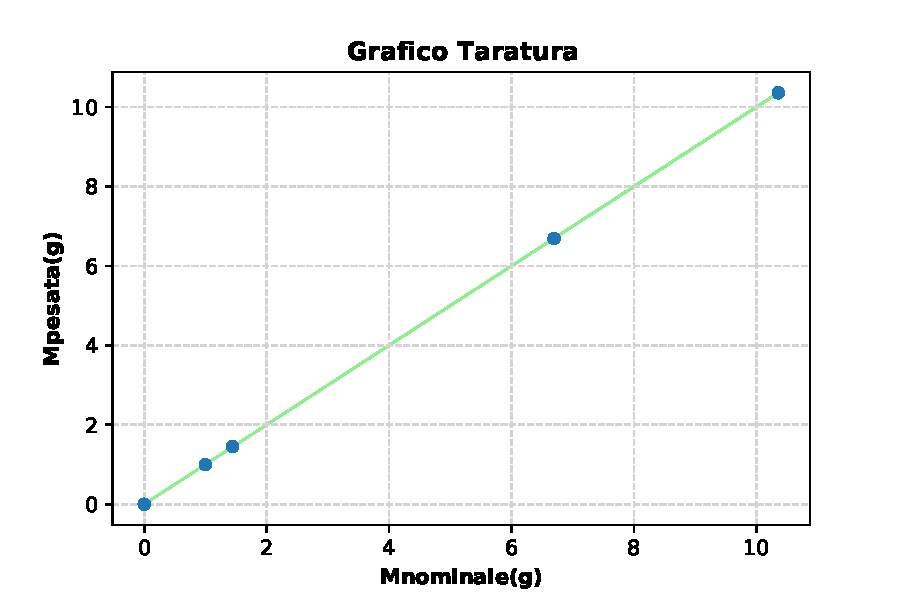
\includegraphics[width=13.5cm]{Figures/Grafico_Taratura.pdf}
  \caption{Grafico della massa pesata sulla massa nominale (entrambe in grammi). L'errore sulla massa nominale è stato considerato trascurabile, mentre l'errore sulla massa pesata è 0.01g. L'andamento è lineare e con pendenza $1$ come ci si aspetta da una bilancia tarata.}   
  \label{fig:GraficoTaratura}
\end{figure}
\par
Da questo grafico è stato possibile ricavare la pendenza attraverso un fit con la seguente formula
\begin{equation*}
    M_{pesata} = \text{pendenza}\cdot M_{nominale}
\end{equation*}
la quale è risultata essere $pendenza = 1.0000 \pm 0.0003$, compatibile con il valore 1. 
\\
In conclusione, la bilancia era tarata opportunamente.
\par}
\subsection{Procedimento Parte I}
{\fontsize{12}{14}\selectfont 

La parte I dell'esperienza consiste nel misurare la forza di Lorentz al variare della corrente. 
\\
Si è prima pesato il magnete A sulla bilancia, ottenendo una misura di $M_{0A} = (158.30 \pm 0.01)g$, poi è stata montata la Current Balance Main Unit con il circuito SF42 in quanto è il più lungo dei circuiti stampati, nonchè quello con il minore errore relativo sulla lunghezza.
Il circuito è stato inserito nel magnete in modo tale da formare un angolo di 90° rispetto al campo magnetico, avendo cura di non metterli a contatto.
\\
Dopo aver acceso il generatore in modalità corrente ed averlo impostato a 0A è stato montato il circuito nel modo seguente:

\par
\begin{center}
    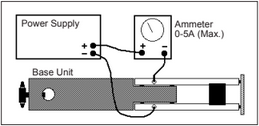
\includegraphics[width=8cm]{Figures/Circuito.png}
\end{center}
\par

Quindi è stato misurato il peso del magnete al variare della corrente a passi di $0.5$A fino ad arrivare a $4.5$A per non superare la portata di 5A dell'amperometro. 
\\
Per verificare la ripetibilità delle misure, il circuito è stato completamente smontato e ricostruito prima di prendere un secondo set.
\\
Ogni misura è stata sottratta al peso $M_{0A}$ per ricavare la variazione di peso dovuta alla forza di Lorentz ed è poi stata plottata in funzione della corrente.
\par}
\subsection{Procedimento Parte II}
{\fontsize{12}{14}\selectfont 


La parte II dell'esperienza consiste nel misurare la forza di Lorentz in funzione della lunghezza del circuito: dopo aver montato la strumentazione come nella parte I, è stata fissata la corrente a $ (3 \pm 0.1) A$ misurando il peso del magnete al variare del circuito stampato.
La differenza della massa pesata con $M_{0A}$ è stata poi plottata in funzione della lunghezza del circuito nel grafico [\ref{fig:GraficoParteII}]


\par}

\subsection{Procedimento Parte III}
{\fontsize{12}{14}\selectfont 

La parte III dell'esperienza consiste nel misurare la forza di Lorentz in funzione dell'angolo $\theta$. L'apparato è stato montato come negli esperimenti precedenti, aggiungendo l'\emph{accessory unit} e rimuovendo il circuito stampato. È stato inoltre utilizzato il magnete B.
\par
Scelto come valore della corrente $(1 \pm 0.1) A$, come in precedenza è stata misurata la massa del magnete mentre l'amperometro segnava 0A ottenendo $M_{0B}' = (70.76 \pm 0.01) g$. Il generatore tuttavia riportava una corrente di 0.02A, quindi la misura è stata replicata a circuito aperto ottenendo $M_{0B} = (70.735 \pm 0.01) g$.
\par
Le misure sono state fatte ogni 20° in tutto il range di 200° dell'accessory unit. Terminato il primo set è stato ruotato il magnete di circa 180°, prendendo nuove misure con lo stesso passo. Questo ha fatto sì che i punti dei due set si sovrapponessero in un breve tratto, così da facilitare l'unione in un unico set che contenesse 2 picchi.
\par
Plottando le differenze di peso in funzione dell'angolo è stato fatto un fit per ognuno dei due set; la funzione fittata è stata $y = A\cdot \sin(\omega t + \phi)$.
\\
I due set sono stati traslati della loro fase in modo da unirli in un unico set. Tuttavia i punti non si sono sovrapposti come atteso, per cui è stato ulteriormente traslato ad occhio il secondo set di misure, fino ad ottenere una perfetta sovrapposizione dei dati. Come errore su questa procedura è stato considerato $2\delta_{M}$, ovvero la distanza massima entro la quale si potevano trovare i punti. Questo errore, sommato in quadratura all'errore iniziale di 0.02g, è diventato $\delta_M = 0.04g$.

\par}
\newpage
\section{Risultati}
\subsection{Risultati Parte I}\label{sec:risultati 1}
{\fontsize{12}{14}\selectfont 
\begin{figure}[H]
  \centering
  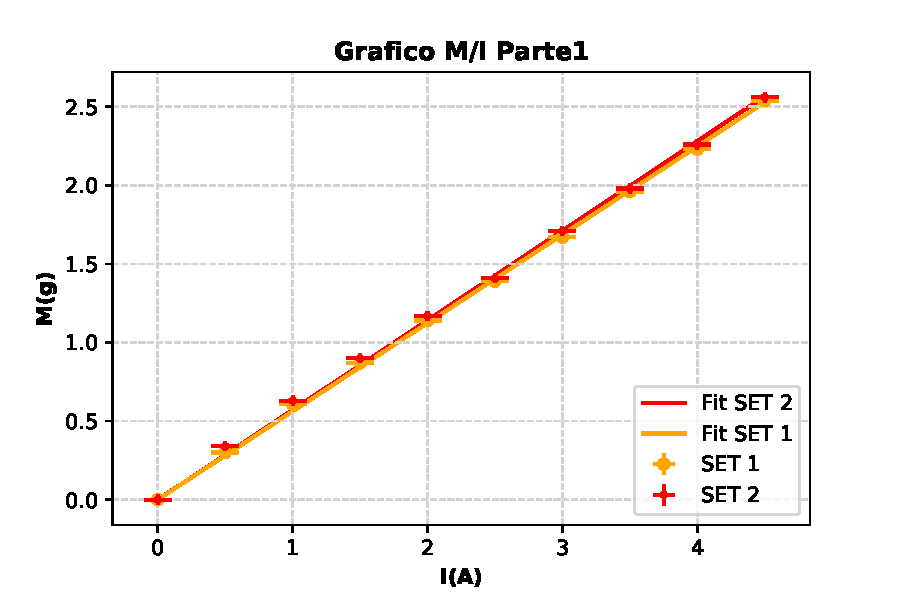
\includegraphics[width=15cm]{Figures/GraficoMIParte1.pdf}
  \caption{Grafico della differenza di massa (in grammi) in funzione della corrente (in Ampere) per due set differenti. La variazione di massa è stata ottenuta come differenza tra la massa pesata e quella a circuito aperto e gli è stato attribuito un errore di $0.02g$ ottenuto da una somma diretta degli errori sulle singole pesate. Per l'errore della corrente è stato considerato un errore del 2\% sul f.s., quindi di 0.1A. Si nota un andamento dei dati lineare compatibilmente con la formula [\ref{eq:FL}] e con il fit usato, della forma $M = pendenza \cdot I$ quindi passante per lo 0. Inoltre dai due set si evidenzia la ripetibilità delle misure.}   
  \label{fig:GraficoParteI}
\end{figure}

Dai set di dati ci è stato inoltre possibile ricavare il campo magnetico $B$ del magnete A dalla formula [\ref{eq:FL}], facendo quindi una media pesata e calcolando una sigma per entrambi i set si è ottenuto:

\par
\begin{equation*}
    B_{SET1} = (7.0 \pm 0.3)\cdot 10^{-2}T
\end{equation*}

\begin{equation*}
    B_{SET2} = (7.4 \pm 0.6)\cdot 10^{-2}T 
\end{equation*}

%Ed infine incrociando i valori ottenuti dai due set, compatibili tra di loro, è stato ottenuto il risultato finale del campo magnetico, il cui risultato aprossimato è:


\begin{figure}[H]
  \centering
  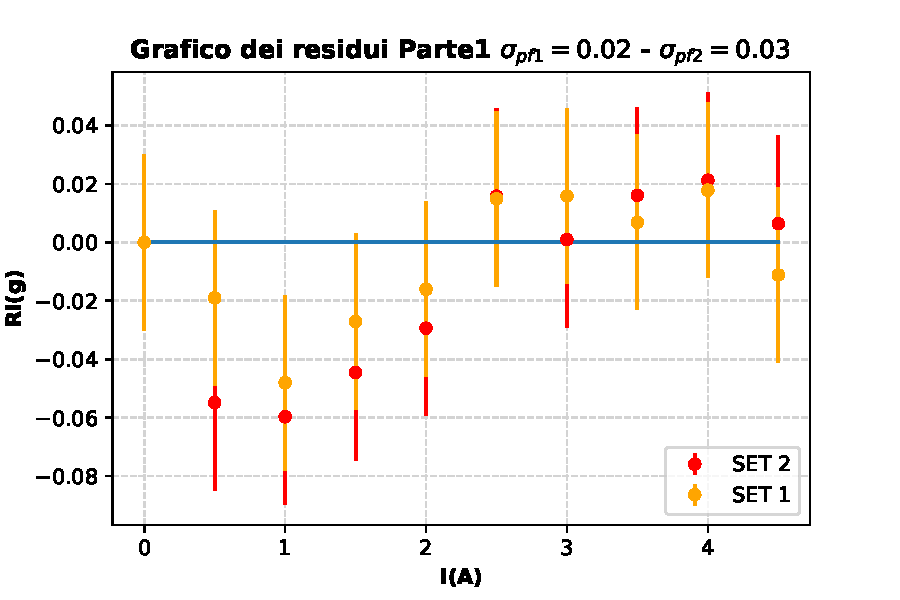
\includegraphics[width=13.5cm]{Figures/Residui_Parte1.pdf}
  \caption{Grafico dei residui corrispondente al set di dati del grafico [\ref{fig:GraficoParteI}], come si nota i residui dei due set sembrano avere un andamento comune, questo potrebbe essere  casuale oppure dovuto al fatto che le misure sono state prese nello stesso ordine in entrambi i set.}   
  \label{fig:GraficoResiduiParteI}
\end{figure}
\par}

\subsection{Risultati Parte II}
{\fontsize{12}{18}\selectfont 

\begin{figure}[H]
  \centering
  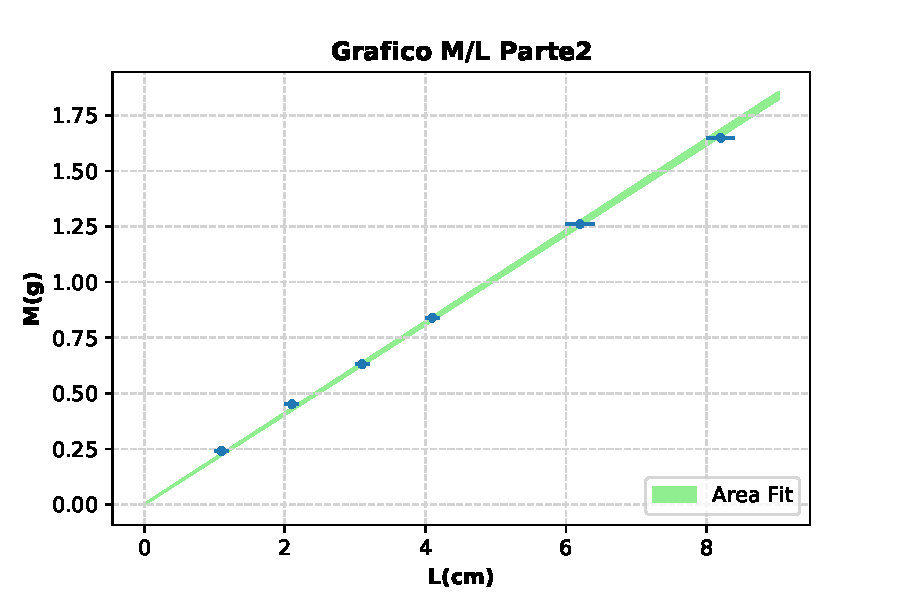
\includegraphics[width=13.5cm]{Figures/GraficoMLParte2.pdf}
  \caption{Grafico della differenza di massa in grammi in funzione della lunghezza del circuito stampato L in metri. La variazione di massa è stata ottenuta come differenza con la massa a circuito aperto e gli è stato attribuito un errore di $0.02g$ ottenuto da una somma diretta degli errori sulle singole pesate. I circuiti stampati erano percorsi da una corrente fissata di 3A. Per l'errore sulla lunghezza dei circuiti si è fatto riferimento al manuale come illustrato nella strumentazione. Si nota un andamento dei dati lineare compatibilmente con la formula [\ref{eq:FL}] e con il fit usato, della forma $M = pendenza \cdot L$ quindi passante per lo 0. L'area di fit è quella compresa tra le rette di massima e di minima pendenza.}   
  \label{fig:GraficoParteII}
\end{figure}
Da questo set di dati ci è stato possibile ricavare nuovamente il campo magnetico B del magnete A, facendo quindi una media pesata e calcolando la deviazione standard si è ottenuto il risultato:

\par
\begin{equation*}
    B_{SET3} = (6.9 \pm 0.3)\cdot 10^{-2}T
\end{equation*}
Questo valore di B e quelli calcolati nella parte I risultano compatibili tra di loro, è dunque possibile ottnere un valore finale del campo magnetico pari a:
3
\begin{equation*}
    B = (7.05 \pm 0.15)\cdot 10^{-2}T 
\end{equation*}

\par}

\subsection{Risultati Parte III}
{\fontsize{12}{14}\selectfont 

\begin{figure}[H]
  \centering
  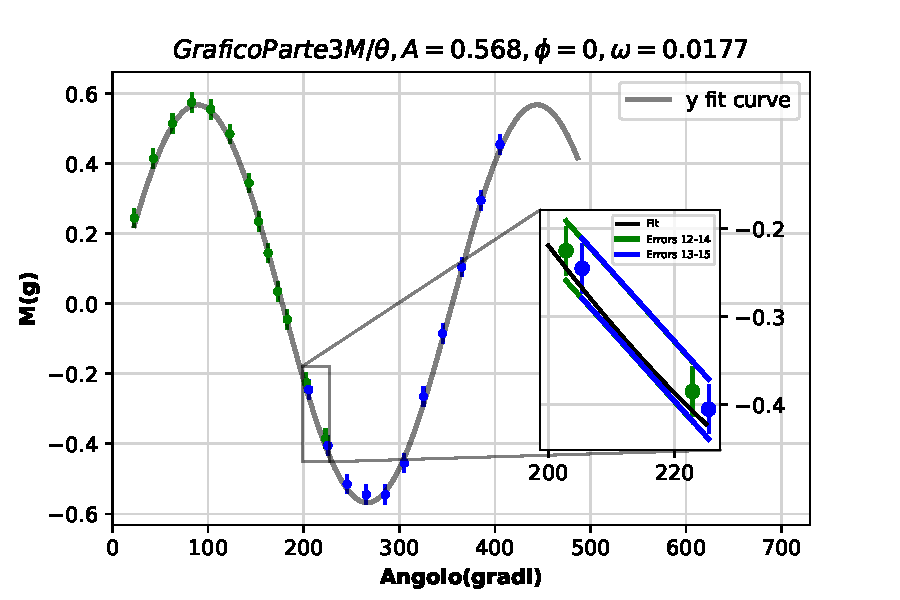
\includegraphics[width=15cm]{Figures/GraficoMthetaParte3.pdf}
  \caption{Grafico della differenza di massa (in grammi) in funzione dell'angolo $\theta$ (in gradi). La variazione di massa è stata ottenuta come differenza tra la massa pesata e quella a circuito aperto e gli è stato attribuito un errore di $0.02g$ ottenuto da una somma diretta degli errori sulle singole pesate. Le misure sono state prese facendo ruotare il circuito dell'\emph{accessory unit} a corrente fissata di 1A. Per l'errore sull'angolo è stata presa mezza tacca sul goniometro, ovvero 0.5°.
  Si nota un andamento sinusoidale compatibilmente con la formula [\ref{eq:FL}].}   
  \label{fig:GraficoParteIII}
\end{figure}
I valori di ampiezza, fase e frequenza sono stati ricavati dal fit $M = A \cdot sin(\omega \cdot t + \phi)$; l'errore di ciascun parametro è stato stimato variando manualmente il suo valore in modo che la curva rientrasse nelle barre di errore dei dati.

\begin{equation*}
    A = (0.568 \pm 0.005) g \qquad \phi = (0.00 \pm 0.02) \text{rad} \qquad \omega = (0.01768 \pm 0.00008)\text{rad}/s %review
\end{equation*}

\par}
\newpage
\subsection{Risultati Lunghezza filo Parte III}
{\fontsize{12}{14}\selectfont 

Per calcolare la lunghezza del circuito dell'\emph{accessory unit} immerso nel campo magnetico è stato misurato con il calibro il lato di una spira, ottenendo $(1.16 \pm 0.01) cm$. Questo valore è stato poi moltiplicato per il numero di spire (n=11), ottenendo $(12.76 \pm 0.11) cm$. %review
\\
%Poi con l'utilizzo della strumentazione sono stati presi due set di misure, uno al variare della corrente con angolo fissato a 90° ed uno al variare dell'angolo con corrente fissata a 1.5A. Oltre a questi due set è stato considerato il set della parte III come secondo set con corrente fissata ed angolo variabile. 
\\
%È stato calcolato il prodotto $LB$ facendo una media pesata e calcolandone la sigma.

%\begin{align*}
    %LB_1 &= (5.2 \pm 0.3)\cdot 10^{-3} T \cdot m \\
    %LB_2 &= (5.31 \pm 0.17)\cdot 10^{-3} T \cdot m \\
    %LB_3 &= (5.4 \pm 0.2)\cdot 10^{-3} T \cdot m 
%\end{align*}

%Si è proceduto sostituendo al primo set il valore di $L$ ottenuto dal calibro ottenendo:

%\begin{equation*}
 %   B = (4.1 \pm 0.2) \cdot 10^{-2} T
%\end{equation*}

%Nei due set ad angolo variabile è stato sostituito questo valore $B$, ottenendo due valori di $L$; infine facendo una media pesata si è riusciti ad ottenere il risultato finale di $L$ come:

%\begin{equation*}
    %L = (12.90 \pm 0.08) cm
%\end{equation*}

\par}
\section{Conclusioni}
{\fontsize{12}{14}\selectfont 

Grazie a questo esperimento è stato verificato con successo che la forza di Lorentz dipende linearmente dalla lunghezza del filo $L$, dalla corrente che attraversa il circuito $I$ e dal seno dell'angolo $\theta$ tra il circuito ed il campo magnetico.
\par
Ripetendo l'esperimento sarebbe opportuno prendere le misure di ogni set in ordine aleatorio, in modo da evitare andamenti periodici negli errori dovuti a variazioni, nel tempo, della risposta degli strumenti
\par
Inoltre nella parte III sarebbe stato opportuno sovrapporre più dati tra i due set, ruotando di qualche grado in meno il magnete prima di passare al set successivo, così da avere una ricucitura più efficace.

\par}
\end{document}